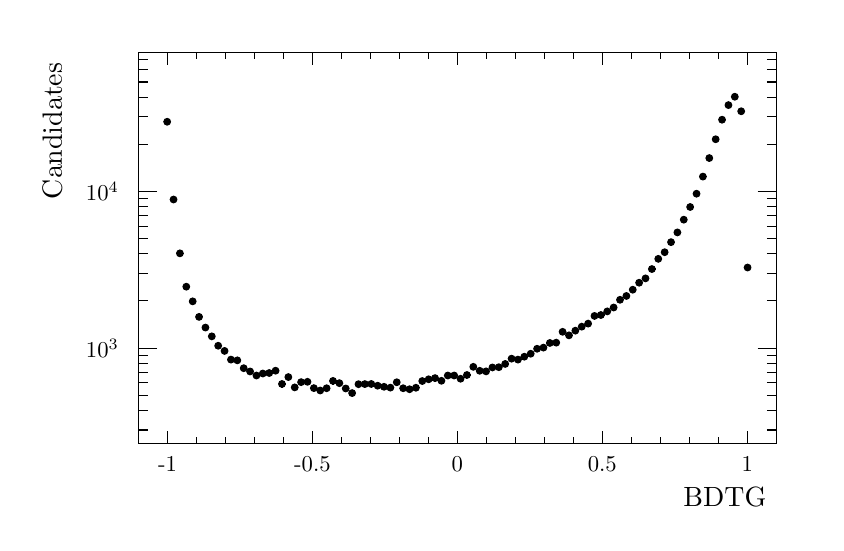
\begin{tikzpicture}
\pgfdeclareplotmark{cross} {
\pgfpathmoveto{\pgfpoint{-0.3\pgfplotmarksize}{\pgfplotmarksize}}
\pgfpathlineto{\pgfpoint{+0.3\pgfplotmarksize}{\pgfplotmarksize}}
\pgfpathlineto{\pgfpoint{+0.3\pgfplotmarksize}{0.3\pgfplotmarksize}}
\pgfpathlineto{\pgfpoint{+1\pgfplotmarksize}{0.3\pgfplotmarksize}}
\pgfpathlineto{\pgfpoint{+1\pgfplotmarksize}{-0.3\pgfplotmarksize}}
\pgfpathlineto{\pgfpoint{+0.3\pgfplotmarksize}{-0.3\pgfplotmarksize}}
\pgfpathlineto{\pgfpoint{+0.3\pgfplotmarksize}{-1.\pgfplotmarksize}}
\pgfpathlineto{\pgfpoint{-0.3\pgfplotmarksize}{-1.\pgfplotmarksize}}
\pgfpathlineto{\pgfpoint{-0.3\pgfplotmarksize}{-0.3\pgfplotmarksize}}
\pgfpathlineto{\pgfpoint{-1.\pgfplotmarksize}{-0.3\pgfplotmarksize}}
\pgfpathlineto{\pgfpoint{-1.\pgfplotmarksize}{0.3\pgfplotmarksize}}
\pgfpathlineto{\pgfpoint{-0.3\pgfplotmarksize}{0.3\pgfplotmarksize}}
\pgfpathclose
\pgfusepathqstroke
}
\pgfdeclareplotmark{cross*} {
\pgfpathmoveto{\pgfpoint{-0.3\pgfplotmarksize}{\pgfplotmarksize}}
\pgfpathlineto{\pgfpoint{+0.3\pgfplotmarksize}{\pgfplotmarksize}}
\pgfpathlineto{\pgfpoint{+0.3\pgfplotmarksize}{0.3\pgfplotmarksize}}
\pgfpathlineto{\pgfpoint{+1\pgfplotmarksize}{0.3\pgfplotmarksize}}
\pgfpathlineto{\pgfpoint{+1\pgfplotmarksize}{-0.3\pgfplotmarksize}}
\pgfpathlineto{\pgfpoint{+0.3\pgfplotmarksize}{-0.3\pgfplotmarksize}}
\pgfpathlineto{\pgfpoint{+0.3\pgfplotmarksize}{-1.\pgfplotmarksize}}
\pgfpathlineto{\pgfpoint{-0.3\pgfplotmarksize}{-1.\pgfplotmarksize}}
\pgfpathlineto{\pgfpoint{-0.3\pgfplotmarksize}{-0.3\pgfplotmarksize}}
\pgfpathlineto{\pgfpoint{-1.\pgfplotmarksize}{-0.3\pgfplotmarksize}}
\pgfpathlineto{\pgfpoint{-1.\pgfplotmarksize}{0.3\pgfplotmarksize}}
\pgfpathlineto{\pgfpoint{-0.3\pgfplotmarksize}{0.3\pgfplotmarksize}}
\pgfpathclose
\pgfusepathqfillstroke
}
\pgfdeclareplotmark{newstar} {
\pgfpathmoveto{\pgfqpoint{0pt}{\pgfplotmarksize}}
\pgfpathlineto{\pgfqpointpolar{44}{0.5\pgfplotmarksize}}
\pgfpathlineto{\pgfqpointpolar{18}{\pgfplotmarksize}}
\pgfpathlineto{\pgfqpointpolar{-20}{0.5\pgfplotmarksize}}
\pgfpathlineto{\pgfqpointpolar{-54}{\pgfplotmarksize}}
\pgfpathlineto{\pgfqpointpolar{-90}{0.5\pgfplotmarksize}}
\pgfpathlineto{\pgfqpointpolar{234}{\pgfplotmarksize}}
\pgfpathlineto{\pgfqpointpolar{198}{0.5\pgfplotmarksize}}
\pgfpathlineto{\pgfqpointpolar{162}{\pgfplotmarksize}}
\pgfpathlineto{\pgfqpointpolar{134}{0.5\pgfplotmarksize}}
\pgfpathclose
\pgfusepathqstroke
}
\pgfdeclareplotmark{newstar*} {
\pgfpathmoveto{\pgfqpoint{0pt}{\pgfplotmarksize}}
\pgfpathlineto{\pgfqpointpolar{44}{0.5\pgfplotmarksize}}
\pgfpathlineto{\pgfqpointpolar{18}{\pgfplotmarksize}}
\pgfpathlineto{\pgfqpointpolar{-20}{0.5\pgfplotmarksize}}
\pgfpathlineto{\pgfqpointpolar{-54}{\pgfplotmarksize}}
\pgfpathlineto{\pgfqpointpolar{-90}{0.5\pgfplotmarksize}}
\pgfpathlineto{\pgfqpointpolar{234}{\pgfplotmarksize}}
\pgfpathlineto{\pgfqpointpolar{198}{0.5\pgfplotmarksize}}
\pgfpathlineto{\pgfqpointpolar{162}{\pgfplotmarksize}}
\pgfpathlineto{\pgfqpointpolar{134}{0.5\pgfplotmarksize}}
\pgfpathclose
\pgfusepathqfillstroke
}
\definecolor{c}{rgb}{1,1,1};
\draw [color=c, fill=c] (0,0) rectangle (10,6.27517);
\draw [color=c, fill=c] (1.4,1.00403) rectangle (9.5,5.96141);
\definecolor{c}{rgb}{0,0,0};
\draw [c] (1.4,1.00403) -- (1.4,5.96141) -- (9.5,5.96141) -- (9.5,1.00403) -- (1.4,1.00403);
\draw [c,line width=0.4] (1.724,5.08731) -- (1.73094,5.08731);
\draw [c,line width=0.4] (1.79806,5.08731) -- (1.805,5.08731);
\foreach \P in {(1.7645,5.08731)}{\draw[mark options={color=c,fill=c},mark size=1.201201pt,mark=*] plot coordinates {\P};}
\draw [c,line width=0.4] (1.805,4.09981) -- (1.81194,4.09981);
\draw [c,line width=0.4] (1.87906,4.09981) -- (1.886,4.09981);
\foreach \P in {(1.8455,4.09981)}{\draw[mark options={color=c,fill=c},mark size=1.201201pt,mark=*] plot coordinates {\P};}
\draw [c,line width=0.4] (1.886,3.41623) -- (1.89294,3.41623);
\draw [c,line width=0.4] (1.96006,3.41623) -- (1.967,3.41623);
\foreach \P in {(1.9265,3.41623)}{\draw[mark options={color=c,fill=c},mark size=1.201201pt,mark=*] plot coordinates {\P};}
\draw [c,line width=0.4] (1.967,2.99264) -- (1.97394,2.99264);
\draw [c,line width=0.4] (2.04106,2.99264) -- (2.048,2.99264);
\foreach \P in {(2.0075,2.99264)}{\draw[mark options={color=c,fill=c},mark size=1.201201pt,mark=*] plot coordinates {\P};}
\draw [c,line width=0.4] (2.048,2.80654) -- (2.05494,2.80654);
\draw [c,line width=0.4] (2.12206,2.80654) -- (2.129,2.80654);
\foreach \P in {(2.0885,2.80654)}{\draw[mark options={color=c,fill=c},mark size=1.201201pt,mark=*] plot coordinates {\P};}
\draw [c,line width=0.4] (2.129,2.60923) -- (2.13594,2.60923);
\draw [c,line width=0.4] (2.20306,2.60923) -- (2.21,2.60923);
\foreach \P in {(2.1695,2.60923)}{\draw[mark options={color=c,fill=c},mark size=1.201201pt,mark=*] plot coordinates {\P};}
\draw [c,line width=0.4] (2.21,2.47354) -- (2.21694,2.47354);
\draw [c,line width=0.4] (2.28406,2.47354) -- (2.291,2.47354);
\foreach \P in {(2.2505,2.47354)}{\draw[mark options={color=c,fill=c},mark size=1.201201pt,mark=*] plot coordinates {\P};}
\draw [c,line width=0.4] (2.291,2.36185) -- (2.29794,2.36185);
\draw [c,line width=0.4] (2.36506,2.36185) -- (2.372,2.36185);
\foreach \P in {(2.3315,2.36185)}{\draw[mark options={color=c,fill=c},mark size=1.201201pt,mark=*] plot coordinates {\P};}
\draw [c,line width=0.4] (2.372,2.24277) -- (2.37894,2.24277);
\draw [c,line width=0.4] (2.44606,2.24277) -- (2.453,2.24277);
\foreach \P in {(2.4125,2.24277)}{\draw[mark options={color=c,fill=c},mark size=1.201201pt,mark=*] plot coordinates {\P};}
\draw [c,line width=0.4] (2.453,2.1769) -- (2.45994,2.1769);
\draw [c,line width=0.4] (2.52706,2.1769) -- (2.534,2.1769);
\foreach \P in {(2.4935,2.1769)}{\draw[mark options={color=c,fill=c},mark size=1.201201pt,mark=*] plot coordinates {\P};}
\draw [c,line width=0.4] (2.534,2.06657) -- (2.54094,2.06657);
\draw [c,line width=0.4] (2.60806,2.06657) -- (2.615,2.06657);
\foreach \P in {(2.5745,2.06657)}{\draw[mark options={color=c,fill=c},mark size=1.201201pt,mark=*] plot coordinates {\P};}
\draw [c,line width=0.4] (2.615,2.05731) -- (2.62194,2.05731);
\draw [c,line width=0.4] (2.68906,2.05731) -- (2.696,2.05731);
\foreach \P in {(2.6555,2.05731)}{\draw[mark options={color=c,fill=c},mark size=1.201201pt,mark=*] plot coordinates {\P};}
\draw [c,line width=0.4] (2.696,1.95765) -- (2.70294,1.95765);
\draw [c,line width=0.4] (2.77006,1.95765) -- (2.777,1.95765);
\foreach \P in {(2.7365,1.95765)}{\draw[mark options={color=c,fill=c},mark size=1.201201pt,mark=*] plot coordinates {\P};}
\draw [c,line width=0.4] (2.777,1.91603) -- (2.78394,1.91603);
\draw [c,line width=0.4] (2.85106,1.91603) -- (2.858,1.91603);
\foreach \P in {(2.8175,1.91603)}{\draw[mark options={color=c,fill=c},mark size=1.201201pt,mark=*] plot coordinates {\P};}
\draw [c,line width=0.4] (2.8985,1.8305) -- (2.8985,1.83103);
\draw [c,line width=0.4] (2.858,1.86458) -- (2.86494,1.86458);
\draw [c,line width=0.4] (2.93206,1.86458) -- (2.939,1.86458);
\foreach \P in {(2.8985,1.86458)}{\draw[mark options={color=c,fill=c},mark size=1.201201pt,mark=*] plot coordinates {\P};}
\draw [c,line width=0.4] (2.9795,1.85649) -- (2.9795,1.85651);
\draw [c,line width=0.4] (2.939,1.89006) -- (2.94594,1.89006);
\draw [c,line width=0.4] (3.01306,1.89006) -- (3.02,1.89006);
\foreach \P in {(2.9795,1.89006)}{\draw[mark options={color=c,fill=c},mark size=1.201201pt,mark=*] plot coordinates {\P};}
\draw [c,line width=0.4] (3.02,1.89632) -- (3.02694,1.89632);
\draw [c,line width=0.4] (3.09406,1.89632) -- (3.101,1.89632);
\foreach \P in {(3.0605,1.89632)}{\draw[mark options={color=c,fill=c},mark size=1.201201pt,mark=*] plot coordinates {\P};}
\draw [c,line width=0.4] (3.101,1.92572) -- (3.10794,1.92572);
\draw [c,line width=0.4] (3.17506,1.92572) -- (3.182,1.92572);
\foreach \P in {(3.1415,1.92572)}{\draw[mark options={color=c,fill=c},mark size=1.201201pt,mark=*] plot coordinates {\P};}
\draw [c,line width=0.4] (3.2225,1.72103) -- (3.2225,1.72378);
\draw [c,line width=0.4] (3.2225,1.7909) -- (3.2225,1.79219);
\draw [c,line width=0.4] (3.182,1.75734) -- (3.18894,1.75734);
\draw [c,line width=0.4] (3.25606,1.75734) -- (3.263,1.75734);
\foreach \P in {(3.2225,1.75734)}{\draw[mark options={color=c,fill=c},mark size=1.201201pt,mark=*] plot coordinates {\P};}
\draw [c,line width=0.4] (3.3035,1.81049) -- (3.3035,1.81141);
\draw [c,line width=0.4] (3.263,1.84497) -- (3.26994,1.84497);
\draw [c,line width=0.4] (3.33706,1.84497) -- (3.344,1.84497);
\foreach \P in {(3.3035,1.84497)}{\draw[mark options={color=c,fill=c},mark size=1.201201pt,mark=*] plot coordinates {\P};}
\draw [c,line width=0.4] (3.3845,1.67655) -- (3.3845,1.68025);
\draw [c,line width=0.4] (3.3845,1.74736) -- (3.3845,1.74952);
\draw [c,line width=0.4] (3.344,1.71381) -- (3.35094,1.71381);
\draw [c,line width=0.4] (3.41806,1.71381) -- (3.425,1.71381);
\foreach \P in {(3.3845,1.71381)}{\draw[mark options={color=c,fill=c},mark size=1.201201pt,mark=*] plot coordinates {\P};}
\draw [c,line width=0.4] (3.4655,1.74463) -- (3.4655,1.74689);
\draw [c,line width=0.4] (3.4655,1.81401) -- (3.4655,1.81484);
\draw [c,line width=0.4] (3.425,1.78045) -- (3.43194,1.78045);
\draw [c,line width=0.4] (3.49906,1.78045) -- (3.506,1.78045);
\foreach \P in {(3.4655,1.78045)}{\draw[mark options={color=c,fill=c},mark size=1.201201pt,mark=*] plot coordinates {\P};}
\draw [c,line width=0.4] (3.5465,1.74899) -- (3.5465,1.75116);
\draw [c,line width=0.4] (3.5465,1.81827) -- (3.5465,1.81902);
\draw [c,line width=0.4] (3.506,1.78472) -- (3.51294,1.78472);
\draw [c,line width=0.4] (3.58006,1.78472) -- (3.587,1.78472);
\foreach \P in {(3.5465,1.78472)}{\draw[mark options={color=c,fill=c},mark size=1.201201pt,mark=*] plot coordinates {\P};}
\draw [c,line width=0.4] (3.6275,1.66706) -- (3.6275,1.67096);
\draw [c,line width=0.4] (3.6275,1.73808) -- (3.6275,1.74043);
\draw [c,line width=0.4] (3.587,1.70452) -- (3.59394,1.70452);
\draw [c,line width=0.4] (3.66106,1.70452) -- (3.668,1.70452);
\foreach \P in {(3.6275,1.70452)}{\draw[mark options={color=c,fill=c},mark size=1.201201pt,mark=*] plot coordinates {\P};}
\draw [c,line width=0.4] (3.7085,1.6363) -- (3.7085,1.64088);
\draw [c,line width=0.4] (3.7085,1.70799) -- (3.7085,1.71096);
\draw [c,line width=0.4] (3.668,1.67443) -- (3.67494,1.67443);
\draw [c,line width=0.4] (3.74206,1.67443) -- (3.749,1.67443);
\foreach \P in {(3.7085,1.67443)}{\draw[mark options={color=c,fill=c},mark size=1.201201pt,mark=*] plot coordinates {\P};}
\draw [c,line width=0.4] (3.7895,1.66546) -- (3.7895,1.66941);
\draw [c,line width=0.4] (3.7895,1.73652) -- (3.7895,1.7389);
\draw [c,line width=0.4] (3.749,1.70296) -- (3.75594,1.70296);
\draw [c,line width=0.4] (3.82306,1.70296) -- (3.83,1.70296);
\foreach \P in {(3.7895,1.70296)}{\draw[mark options={color=c,fill=c},mark size=1.201201pt,mark=*] plot coordinates {\P};}
\draw [c,line width=0.4] (3.8705,1.7605) -- (3.8705,1.76243);
\draw [c,line width=0.4] (3.8705,1.82954) -- (3.8705,1.83008);
\draw [c,line width=0.4] (3.83,1.79599) -- (3.83694,1.79599);
\draw [c,line width=0.4] (3.90406,1.79599) -- (3.911,1.79599);
\foreach \P in {(3.8705,1.79599)}{\draw[mark options={color=c,fill=c},mark size=1.201201pt,mark=*] plot coordinates {\P};}
\draw [c,line width=0.4] (3.9515,1.73143) -- (3.9515,1.73397);
\draw [c,line width=0.4] (3.9515,1.80108) -- (3.9515,1.80217);
\draw [c,line width=0.4] (3.911,1.76753) -- (3.91794,1.76753);
\draw [c,line width=0.4] (3.98506,1.76753) -- (3.992,1.76753);
\foreach \P in {(3.9515,1.76753)}{\draw[mark options={color=c,fill=c},mark size=1.201201pt,mark=*] plot coordinates {\P};}
\draw [c,line width=0.4] (4.0325,1.66227) -- (4.0325,1.66628);
\draw [c,line width=0.4] (4.0325,1.7334) -- (4.0325,1.73584);
\draw [c,line width=0.4] (3.992,1.69984) -- (3.99894,1.69984);
\draw [c,line width=0.4] (4.06606,1.69984) -- (4.073,1.69984);
\foreach \P in {(4.0325,1.69984)}{\draw[mark options={color=c,fill=c},mark size=1.201201pt,mark=*] plot coordinates {\P};}
\draw [c,line width=0.4] (4.1135,1.6027) -- (4.1135,1.60803);
\draw [c,line width=0.4] (4.1135,1.67515) -- (4.1135,1.6788);
\draw [c,line width=0.4] (4.073,1.64159) -- (4.07994,1.64159);
\draw [c,line width=0.4] (4.14706,1.64159) -- (4.154,1.64159);
\foreach \P in {(4.1135,1.64159)}{\draw[mark options={color=c,fill=c},mark size=1.201201pt,mark=*] plot coordinates {\P};}
\draw [c,line width=0.4] (4.1945,1.71803) -- (4.1945,1.72085);
\draw [c,line width=0.4] (4.1945,1.78796) -- (4.1945,1.78931);
\draw [c,line width=0.4] (4.154,1.75441) -- (4.16094,1.75441);
\draw [c,line width=0.4] (4.22806,1.75441) -- (4.235,1.75441);
\foreach \P in {(4.1945,1.75441)}{\draw[mark options={color=c,fill=c},mark size=1.201201pt,mark=*] plot coordinates {\P};}
\draw [c,line width=0.4] (4.2755,1.71953) -- (4.2755,1.72232);
\draw [c,line width=0.4] (4.2755,1.78943) -- (4.2755,1.79075);
\draw [c,line width=0.4] (4.235,1.75587) -- (4.24194,1.75587);
\draw [c,line width=0.4] (4.30906,1.75587) -- (4.316,1.75587);
\foreach \P in {(4.2755,1.75587)}{\draw[mark options={color=c,fill=c},mark size=1.201201pt,mark=*] plot coordinates {\P};}
\draw [c,line width=0.4] (4.3565,1.72103) -- (4.3565,1.72378);
\draw [c,line width=0.4] (4.3565,1.7909) -- (4.3565,1.79219);
\draw [c,line width=0.4] (4.316,1.75734) -- (4.32294,1.75734);
\draw [c,line width=0.4] (4.39006,1.75734) -- (4.397,1.75734);
\foreach \P in {(4.3565,1.75734)}{\draw[mark options={color=c,fill=c},mark size=1.201201pt,mark=*] plot coordinates {\P};}
\draw [c,line width=0.4] (4.4375,1.69831) -- (4.4375,1.70154);
\draw [c,line width=0.4] (4.4375,1.76865) -- (4.4375,1.77039);
\draw [c,line width=0.4] (4.397,1.7351) -- (4.40394,1.7351);
\draw [c,line width=0.4] (4.47106,1.7351) -- (4.478,1.7351);
\foreach \P in {(4.4375,1.7351)}{\draw[mark options={color=c,fill=c},mark size=1.201201pt,mark=*] plot coordinates {\P};}
\draw [c,line width=0.4] (4.5185,1.68438) -- (4.5185,1.68791);
\draw [c,line width=0.4] (4.5185,1.75503) -- (4.5185,1.75703);
\draw [c,line width=0.4] (4.478,1.72147) -- (4.48494,1.72147);
\draw [c,line width=0.4] (4.55206,1.72147) -- (4.559,1.72147);
\foreach \P in {(4.5185,1.72147)}{\draw[mark options={color=c,fill=c},mark size=1.201201pt,mark=*] plot coordinates {\P};}
\draw [c,line width=0.4] (4.5995,1.6734) -- (4.5995,1.67717);
\draw [c,line width=0.4] (4.5995,1.74428) -- (4.5995,1.7465);
\draw [c,line width=0.4] (4.559,1.71072) -- (4.56594,1.71072);
\draw [c,line width=0.4] (4.63306,1.71072) -- (4.64,1.71072);
\foreach \P in {(4.5995,1.71072)}{\draw[mark options={color=c,fill=c},mark size=1.201201pt,mark=*] plot coordinates {\P};}
\draw [c,line width=0.4] (4.6805,1.74318) -- (4.6805,1.74547);
\draw [c,line width=0.4] (4.6805,1.81258) -- (4.6805,1.81344);
\draw [c,line width=0.4] (4.64,1.77902) -- (4.64694,1.77902);
\draw [c,line width=0.4] (4.71406,1.77902) -- (4.721,1.77902);
\foreach \P in {(4.6805,1.77902)}{\draw[mark options={color=c,fill=c},mark size=1.201201pt,mark=*] plot coordinates {\P};}
\draw [c,line width=0.4] (4.7615,1.66546) -- (4.7615,1.66941);
\draw [c,line width=0.4] (4.7615,1.73652) -- (4.7615,1.7389);
\draw [c,line width=0.4] (4.721,1.70296) -- (4.72794,1.70296);
\draw [c,line width=0.4] (4.79506,1.70296) -- (4.802,1.70296);
\foreach \P in {(4.7615,1.70296)}{\draw[mark options={color=c,fill=c},mark size=1.201201pt,mark=*] plot coordinates {\P};}
\draw [c,line width=0.4] (4.8425,1.65262) -- (4.8425,1.65684);
\draw [c,line width=0.4] (4.8425,1.72396) -- (4.8425,1.72659);
\draw [c,line width=0.4] (4.802,1.6904) -- (4.80894,1.6904);
\draw [c,line width=0.4] (4.87606,1.6904) -- (4.883,1.6904);
\foreach \P in {(4.8425,1.6904)}{\draw[mark options={color=c,fill=c},mark size=1.201201pt,mark=*] plot coordinates {\P};}
\draw [c,line width=0.4] (4.9235,1.67182) -- (4.9235,1.67562);
\draw [c,line width=0.4] (4.9235,1.74273) -- (4.9235,1.74499);
\draw [c,line width=0.4] (4.883,1.70918) -- (4.88994,1.70918);
\draw [c,line width=0.4] (4.95706,1.70918) -- (4.964,1.70918);
\foreach \P in {(4.9235,1.70918)}{\draw[mark options={color=c,fill=c},mark size=1.201201pt,mark=*] plot coordinates {\P};}
\draw [c,line width=0.4] (5.0045,1.75907) -- (5.0045,1.76103);
\draw [c,line width=0.4] (5.0045,1.82814) -- (5.0045,1.8287);
\draw [c,line width=0.4] (4.964,1.79459) -- (4.97094,1.79459);
\draw [c,line width=0.4] (5.03806,1.79459) -- (5.045,1.79459);
\foreach \P in {(5.0045,1.79459)}{\draw[mark options={color=c,fill=c},mark size=1.201201pt,mark=*] plot coordinates {\P};}
\draw [c,line width=0.4] (5.0855,1.78168) -- (5.0855,1.78318);
\draw [c,line width=0.4] (5.0855,1.85029) -- (5.0855,1.85042);
\draw [c,line width=0.4] (5.045,1.81673) -- (5.05194,1.81673);
\draw [c,line width=0.4] (5.11906,1.81673) -- (5.126,1.81673);
\foreach \P in {(5.0855,1.81673)}{\draw[mark options={color=c,fill=c},mark size=1.201201pt,mark=*] plot coordinates {\P};}
\draw [c,line width=0.4] (5.1665,1.79689) -- (5.1665,1.79808);
\draw [c,line width=0.4] (5.126,1.83164) -- (5.13294,1.83164);
\draw [c,line width=0.4] (5.20006,1.83164) -- (5.207,1.83164);
\foreach \P in {(5.1665,1.83164)}{\draw[mark options={color=c,fill=c},mark size=1.201201pt,mark=*] plot coordinates {\P};}
\draw [c,line width=0.4] (5.2475,1.76192) -- (5.2475,1.76383);
\draw [c,line width=0.4] (5.2475,1.83094) -- (5.2475,1.83145);
\draw [c,line width=0.4] (5.207,1.79739) -- (5.21394,1.79739);
\draw [c,line width=0.4] (5.28106,1.79739) -- (5.288,1.79739);
\foreach \P in {(5.2475,1.79739)}{\draw[mark options={color=c,fill=c},mark size=1.201201pt,mark=*] plot coordinates {\P};}
\draw [c,line width=0.4] (5.3285,1.8305) -- (5.3285,1.83103);
\draw [c,line width=0.4] (5.288,1.86458) -- (5.29494,1.86458);
\draw [c,line width=0.4] (5.36206,1.86458) -- (5.369,1.86458);
\foreach \P in {(5.3285,1.86458)}{\draw[mark options={color=c,fill=c},mark size=1.201201pt,mark=*] plot coordinates {\P};}
\draw [c,line width=0.4] (5.4095,1.8305) -- (5.4095,1.83103);
\draw [c,line width=0.4] (5.369,1.86458) -- (5.37594,1.86458);
\draw [c,line width=0.4] (5.44306,1.86458) -- (5.45,1.86458);
\foreach \P in {(5.4095,1.86458)}{\draw[mark options={color=c,fill=c},mark size=1.201201pt,mark=*] plot coordinates {\P};}
\draw [c,line width=0.4] (5.4905,1.78862) -- (5.4905,1.78998);
\draw [c,line width=0.4] (5.4905,1.8571) -- (5.4905,1.8571);
\draw [c,line width=0.4] (5.45,1.82354) -- (5.45694,1.82354);
\draw [c,line width=0.4] (5.52406,1.82354) -- (5.531,1.82354);
\foreach \P in {(5.4905,1.82354)}{\draw[mark options={color=c,fill=c},mark size=1.201201pt,mark=*] plot coordinates {\P};}
\draw [c,line width=0.4] (5.5715,1.83707) -- (5.5715,1.83747);
\draw [c,line width=0.4] (5.531,1.87102) -- (5.53794,1.87102);
\draw [c,line width=0.4] (5.60506,1.87102) -- (5.612,1.87102);
\foreach \P in {(5.5715,1.87102)}{\draw[mark options={color=c,fill=c},mark size=1.201201pt,mark=*] plot coordinates {\P};}
\draw [c,line width=0.4] (5.612,1.97489) -- (5.61894,1.97489);
\draw [c,line width=0.4] (5.68606,1.97489) -- (5.693,1.97489);
\foreach \P in {(5.6525,1.97489)}{\draw[mark options={color=c,fill=c},mark size=1.201201pt,mark=*] plot coordinates {\P};}
\draw [c,line width=0.4] (5.693,1.92452) -- (5.69994,1.92452);
\draw [c,line width=0.4] (5.76706,1.92452) -- (5.774,1.92452);
\foreach \P in {(5.7335,1.92452)}{\draw[mark options={color=c,fill=c},mark size=1.201201pt,mark=*] plot coordinates {\P};}
\draw [c,line width=0.4] (5.774,1.91725) -- (5.78094,1.91725);
\draw [c,line width=0.4] (5.84806,1.91725) -- (5.855,1.91725);
\foreach \P in {(5.8145,1.91725)}{\draw[mark options={color=c,fill=c},mark size=1.201201pt,mark=*] plot coordinates {\P};}
\draw [c,line width=0.4] (5.855,1.96689) -- (5.86194,1.96689);
\draw [c,line width=0.4] (5.92906,1.96689) -- (5.936,1.96689);
\foreach \P in {(5.8955,1.96689)}{\draw[mark options={color=c,fill=c},mark size=1.201201pt,mark=*] plot coordinates {\P};}
\draw [c,line width=0.4] (5.936,1.97033) -- (5.94294,1.97033);
\draw [c,line width=0.4] (6.01006,1.97033) -- (6.017,1.97033);
\foreach \P in {(5.9765,1.97033)}{\draw[mark options={color=c,fill=c},mark size=1.201201pt,mark=*] plot coordinates {\P};}
\draw [c,line width=0.4] (6.017,2.01165) -- (6.02394,2.01165);
\draw [c,line width=0.4] (6.09106,2.01165) -- (6.098,2.01165);
\foreach \P in {(6.0575,2.01165)}{\draw[mark options={color=c,fill=c},mark size=1.201201pt,mark=*] plot coordinates {\P};}
\draw [c,line width=0.4] (6.098,2.07877) -- (6.10494,2.07877);
\draw [c,line width=0.4] (6.17206,2.07877) -- (6.179,2.07877);
\foreach \P in {(6.1385,2.07877)}{\draw[mark options={color=c,fill=c},mark size=1.201201pt,mark=*] plot coordinates {\P};}
\draw [c,line width=0.4] (6.179,2.06657) -- (6.18594,2.06657);
\draw [c,line width=0.4] (6.25306,2.06657) -- (6.26,2.06657);
\foreach \P in {(6.2195,2.06657)}{\draw[mark options={color=c,fill=c},mark size=1.201201pt,mark=*] plot coordinates {\P};}
\draw [c,line width=0.4] (6.26,2.10363) -- (6.26694,2.10363);
\draw [c,line width=0.4] (6.33406,2.10363) -- (6.341,2.10363);
\foreach \P in {(6.3005,2.10363)}{\draw[mark options={color=c,fill=c},mark size=1.201201pt,mark=*] plot coordinates {\P};}
\draw [c,line width=0.4] (6.341,2.14104) -- (6.34794,2.14104);
\draw [c,line width=0.4] (6.41506,2.14104) -- (6.422,2.14104);
\foreach \P in {(6.3815,2.14104)}{\draw[mark options={color=c,fill=c},mark size=1.201201pt,mark=*] plot coordinates {\P};}
\draw [c,line width=0.4] (6.422,2.20438) -- (6.42894,2.20438);
\draw [c,line width=0.4] (6.49606,2.20438) -- (6.503,2.20438);
\foreach \P in {(6.4625,2.20438)}{\draw[mark options={color=c,fill=c},mark size=1.201201pt,mark=*] plot coordinates {\P};}
\draw [c,line width=0.4] (6.503,2.21909) -- (6.50994,2.21909);
\draw [c,line width=0.4] (6.57706,2.21909) -- (6.584,2.21909);
\foreach \P in {(6.5435,2.21909)}{\draw[mark options={color=c,fill=c},mark size=1.201201pt,mark=*] plot coordinates {\P};}
\draw [c,line width=0.4] (6.584,2.27793) -- (6.59094,2.27793);
\draw [c,line width=0.4] (6.65806,2.27793) -- (6.665,2.27793);
\foreach \P in {(6.6245,2.27793)}{\draw[mark options={color=c,fill=c},mark size=1.201201pt,mark=*] plot coordinates {\P};}
\draw [c,line width=0.4] (6.665,2.28193) -- (6.67194,2.28193);
\draw [c,line width=0.4] (6.73906,2.28193) -- (6.746,2.28193);
\foreach \P in {(6.7055,2.28193)}{\draw[mark options={color=c,fill=c},mark size=1.201201pt,mark=*] plot coordinates {\P};}
\draw [c,line width=0.4] (6.746,2.4195) -- (6.75294,2.4195);
\draw [c,line width=0.4] (6.82006,2.4195) -- (6.827,2.4195);
\foreach \P in {(6.7865,2.4195)}{\draw[mark options={color=c,fill=c},mark size=1.201201pt,mark=*] plot coordinates {\P};}
\draw [c,line width=0.4] (6.827,2.37484) -- (6.83394,2.37484);
\draw [c,line width=0.4] (6.90106,2.37484) -- (6.908,2.37484);
\foreach \P in {(6.8675,2.37484)}{\draw[mark options={color=c,fill=c},mark size=1.201201pt,mark=*] plot coordinates {\P};}
\draw [c,line width=0.4] (6.908,2.43434) -- (6.91494,2.43434);
\draw [c,line width=0.4] (6.98206,2.43434) -- (6.989,2.43434);
\foreach \P in {(6.9485,2.43434)}{\draw[mark options={color=c,fill=c},mark size=1.201201pt,mark=*] plot coordinates {\P};}
\draw [c,line width=0.4] (6.989,2.48497) -- (6.99594,2.48497);
\draw [c,line width=0.4] (7.06306,2.48497) -- (7.07,2.48497);
\foreach \P in {(7.0295,2.48497)}{\draw[mark options={color=c,fill=c},mark size=1.201201pt,mark=*] plot coordinates {\P};}
\draw [c,line width=0.4] (7.07,2.5238) -- (7.07694,2.5238);
\draw [c,line width=0.4] (7.14406,2.5238) -- (7.151,2.5238);
\foreach \P in {(7.1105,2.5238)}{\draw[mark options={color=c,fill=c},mark size=1.201201pt,mark=*] plot coordinates {\P};}
\draw [c,line width=0.4] (7.151,2.62116) -- (7.15794,2.62116);
\draw [c,line width=0.4] (7.22506,2.62116) -- (7.232,2.62116);
\foreach \P in {(7.1915,2.62116)}{\draw[mark options={color=c,fill=c},mark size=1.201201pt,mark=*] plot coordinates {\P};}
\draw [c,line width=0.4] (7.232,2.63293) -- (7.23894,2.63293);
\draw [c,line width=0.4] (7.30606,2.63293) -- (7.313,2.63293);
\foreach \P in {(7.2725,2.63293)}{\draw[mark options={color=c,fill=c},mark size=1.201201pt,mark=*] plot coordinates {\P};}
\draw [c,line width=0.4] (7.313,2.67896) -- (7.31994,2.67896);
\draw [c,line width=0.4] (7.38706,2.67896) -- (7.394,2.67896);
\foreach \P in {(7.3535,2.67896)}{\draw[mark options={color=c,fill=c},mark size=1.201201pt,mark=*] plot coordinates {\P};}
\draw [c,line width=0.4] (7.394,2.72838) -- (7.40094,2.72838);
\draw [c,line width=0.4] (7.46806,2.72838) -- (7.475,2.72838);
\foreach \P in {(7.4345,2.72838)}{\draw[mark options={color=c,fill=c},mark size=1.201201pt,mark=*] plot coordinates {\P};}
\draw [c,line width=0.4] (7.475,2.8263) -- (7.48194,2.8263);
\draw [c,line width=0.4] (7.54906,2.8263) -- (7.556,2.8263);
\foreach \P in {(7.5155,2.8263)}{\draw[mark options={color=c,fill=c},mark size=1.201201pt,mark=*] plot coordinates {\P};}
\draw [c,line width=0.4] (7.556,2.875) -- (7.56294,2.875);
\draw [c,line width=0.4] (7.63006,2.875) -- (7.637,2.875);
\foreach \P in {(7.5965,2.875)}{\draw[mark options={color=c,fill=c},mark size=1.201201pt,mark=*] plot coordinates {\P};}
\draw [c,line width=0.4] (7.637,2.95433) -- (7.64394,2.95433);
\draw [c,line width=0.4] (7.71106,2.95433) -- (7.718,2.95433);
\foreach \P in {(7.6775,2.95433)}{\draw[mark options={color=c,fill=c},mark size=1.201201pt,mark=*] plot coordinates {\P};}
\draw [c,line width=0.4] (7.718,3.04298) -- (7.72494,3.04298);
\draw [c,line width=0.4] (7.79206,3.04298) -- (7.799,3.04298);
\foreach \P in {(7.7585,3.04298)}{\draw[mark options={color=c,fill=c},mark size=1.201201pt,mark=*] plot coordinates {\P};}
\draw [c,line width=0.4] (7.799,3.09802) -- (7.80594,3.09802);
\draw [c,line width=0.4] (7.87306,3.09802) -- (7.88,3.09802);
\foreach \P in {(7.8395,3.09802)}{\draw[mark options={color=c,fill=c},mark size=1.201201pt,mark=*] plot coordinates {\P};}
\draw [c,line width=0.4] (7.88,3.21687) -- (7.88694,3.21687);
\draw [c,line width=0.4] (7.95406,3.21687) -- (7.961,3.21687);
\foreach \P in {(7.9205,3.21687)}{\draw[mark options={color=c,fill=c},mark size=1.201201pt,mark=*] plot coordinates {\P};}
\draw [c,line width=0.4] (7.961,3.34634) -- (7.96794,3.34634);
\draw [c,line width=0.4] (8.03506,3.34634) -- (8.042,3.34634);
\foreach \P in {(8.0015,3.34634)}{\draw[mark options={color=c,fill=c},mark size=1.201201pt,mark=*] plot coordinates {\P};}
\draw [c,line width=0.4] (8.042,3.43069) -- (8.04894,3.43069);
\draw [c,line width=0.4] (8.11606,3.43069) -- (8.123,3.43069);
\foreach \P in {(8.0825,3.43069)}{\draw[mark options={color=c,fill=c},mark size=1.201201pt,mark=*] plot coordinates {\P};}
\draw [c,line width=0.4] (8.123,3.5583) -- (8.12994,3.5583);
\draw [c,line width=0.4] (8.19706,3.5583) -- (8.204,3.5583);
\foreach \P in {(8.1635,3.5583)}{\draw[mark options={color=c,fill=c},mark size=1.201201pt,mark=*] plot coordinates {\P};}
\draw [c,line width=0.4] (8.204,3.68185) -- (8.21094,3.68185);
\draw [c,line width=0.4] (8.27806,3.68185) -- (8.285,3.68185);
\foreach \P in {(8.2445,3.68185)}{\draw[mark options={color=c,fill=c},mark size=1.201201pt,mark=*] plot coordinates {\P};}
\draw [c,line width=0.4] (8.285,3.84372) -- (8.29194,3.84372);
\draw [c,line width=0.4] (8.35906,3.84372) -- (8.366,3.84372);
\foreach \P in {(8.3255,3.84372)}{\draw[mark options={color=c,fill=c},mark size=1.201201pt,mark=*] plot coordinates {\P};}
\draw [c,line width=0.4] (8.366,4.00487) -- (8.37294,4.00487);
\draw [c,line width=0.4] (8.44006,4.00487) -- (8.447,4.00487);
\foreach \P in {(8.4065,4.00487)}{\draw[mark options={color=c,fill=c},mark size=1.201201pt,mark=*] plot coordinates {\P};}
\draw [c,line width=0.4] (8.447,4.17338) -- (8.45394,4.17338);
\draw [c,line width=0.4] (8.52106,4.17338) -- (8.528,4.17338);
\foreach \P in {(8.4875,4.17338)}{\draw[mark options={color=c,fill=c},mark size=1.201201pt,mark=*] plot coordinates {\P};}
\draw [c,line width=0.4] (8.528,4.39075) -- (8.53494,4.39075);
\draw [c,line width=0.4] (8.60206,4.39075) -- (8.609,4.39075);
\foreach \P in {(8.5685,4.39075)}{\draw[mark options={color=c,fill=c},mark size=1.201201pt,mark=*] plot coordinates {\P};}
\draw [c,line width=0.4] (8.609,4.6263) -- (8.61594,4.6263);
\draw [c,line width=0.4] (8.68306,4.6263) -- (8.69,4.6263);
\foreach \P in {(8.6495,4.6263)}{\draw[mark options={color=c,fill=c},mark size=1.201201pt,mark=*] plot coordinates {\P};}
\draw [c,line width=0.4] (8.69,4.86513) -- (8.69694,4.86513);
\draw [c,line width=0.4] (8.76406,4.86513) -- (8.771,4.86513);
\foreach \P in {(8.7305,4.86513)}{\draw[mark options={color=c,fill=c},mark size=1.201201pt,mark=*] plot coordinates {\P};}
\draw [c,line width=0.4] (8.771,5.11325) -- (8.77794,5.11325);
\draw [c,line width=0.4] (8.84506,5.11325) -- (8.852,5.11325);
\foreach \P in {(8.8115,5.11325)}{\draw[mark options={color=c,fill=c},mark size=1.201201pt,mark=*] plot coordinates {\P};}
\draw [c,line width=0.4] (8.852,5.29894) -- (8.85894,5.29894);
\draw [c,line width=0.4] (8.92606,5.29894) -- (8.933,5.29894);
\foreach \P in {(8.8925,5.29894)}{\draw[mark options={color=c,fill=c},mark size=1.201201pt,mark=*] plot coordinates {\P};}
\draw [c,line width=0.4] (8.933,5.40514) -- (8.93994,5.40514);
\draw [c,line width=0.4] (9.00706,5.40514) -- (9.014,5.40514);
\foreach \P in {(8.9735,5.40514)}{\draw[mark options={color=c,fill=c},mark size=1.201201pt,mark=*] plot coordinates {\P};}
\draw [c,line width=0.4] (9.014,5.22045) -- (9.02094,5.22045);
\draw [c,line width=0.4] (9.08806,5.22045) -- (9.095,5.22045);
\foreach \P in {(9.0545,5.22045)}{\draw[mark options={color=c,fill=c},mark size=1.201201pt,mark=*] plot coordinates {\P};}
\draw [c,line width=0.4] (9.095,3.23611) -- (9.10194,3.23611);
\draw [c,line width=0.4] (9.16906,3.23611) -- (9.176,3.23611);
\foreach \P in {(9.1355,3.23611)}{\draw[mark options={color=c,fill=c},mark size=1.201201pt,mark=*] plot coordinates {\P};}
\draw [c,line width=0.4] (1.4,1.00403) -- (9.5,1.00403);
\draw [anchor= east] (9.5,0.317272) node[scale=1.00614, rotate=0]{BDTG};
\draw [c,line width=0.4] (1.76818,1.15651) -- (1.76818,1.00403);
\draw [c,line width=0.4] (2.13636,1.08027) -- (2.13636,1.00403);
\draw [c,line width=0.4] (2.50455,1.08027) -- (2.50455,1.00403);
\draw [c,line width=0.4] (2.87273,1.08027) -- (2.87273,1.00403);
\draw [c,line width=0.4] (3.24091,1.08027) -- (3.24091,1.00403);
\draw [c,line width=0.4] (3.60909,1.15651) -- (3.60909,1.00403);
\draw [c,line width=0.4] (3.97727,1.08027) -- (3.97727,1.00403);
\draw [c,line width=0.4] (4.34545,1.08027) -- (4.34545,1.00403);
\draw [c,line width=0.4] (4.71364,1.08027) -- (4.71364,1.00403);
\draw [c,line width=0.4] (5.08182,1.08027) -- (5.08182,1.00403);
\draw [c,line width=0.4] (5.45,1.15651) -- (5.45,1.00403);
\draw [c,line width=0.4] (5.81818,1.08027) -- (5.81818,1.00403);
\draw [c,line width=0.4] (6.18636,1.08027) -- (6.18636,1.00403);
\draw [c,line width=0.4] (6.55455,1.08027) -- (6.55455,1.00403);
\draw [c,line width=0.4] (6.92273,1.08027) -- (6.92273,1.00403);
\draw [c,line width=0.4] (7.29091,1.15651) -- (7.29091,1.00403);
\draw [c,line width=0.4] (7.65909,1.08027) -- (7.65909,1.00403);
\draw [c,line width=0.4] (8.02727,1.08027) -- (8.02727,1.00403);
\draw [c,line width=0.4] (8.39545,1.08027) -- (8.39545,1.00403);
\draw [c,line width=0.4] (8.76364,1.08027) -- (8.76364,1.00403);
\draw [c,line width=0.4] (9.13182,1.15651) -- (9.13182,1.00403);
\draw [c,line width=0.4] (1.76818,1.15651) -- (1.76818,1.00403);
\draw [c,line width=0.4] (1.4,1.08027) -- (1.4,1.00403);
\draw [c,line width=0.4] (9.13182,1.15651) -- (9.13182,1.00403);
\draw [c,line width=0.4] (9.5,1.08027) -- (9.5,1.00403);
\draw [anchor=base] (1.76818,0.640067) node[scale=0.819821, rotate=0]{-1};
\draw [anchor=base] (3.60909,0.640067) node[scale=0.819821, rotate=0]{-0.5};
\draw [anchor=base] (5.45,0.640067) node[scale=0.819821, rotate=0]{0};
\draw [anchor=base] (7.29091,0.640067) node[scale=0.819821, rotate=0]{0.5};
\draw [anchor=base] (9.13182,0.640067) node[scale=0.819821, rotate=0]{1};
\draw [c,line width=0.4] (1.4,5.96141) -- (9.5,5.96141);
\draw [c,line width=0.4] (1.76818,5.80892) -- (1.76818,5.96141);
\draw [c,line width=0.4] (2.13636,5.88517) -- (2.13636,5.96141);
\draw [c,line width=0.4] (2.50455,5.88517) -- (2.50455,5.96141);
\draw [c,line width=0.4] (2.87273,5.88517) -- (2.87273,5.96141);
\draw [c,line width=0.4] (3.24091,5.88517) -- (3.24091,5.96141);
\draw [c,line width=0.4] (3.60909,5.80892) -- (3.60909,5.96141);
\draw [c,line width=0.4] (3.97727,5.88517) -- (3.97727,5.96141);
\draw [c,line width=0.4] (4.34545,5.88517) -- (4.34545,5.96141);
\draw [c,line width=0.4] (4.71364,5.88517) -- (4.71364,5.96141);
\draw [c,line width=0.4] (5.08182,5.88517) -- (5.08182,5.96141);
\draw [c,line width=0.4] (5.45,5.80892) -- (5.45,5.96141);
\draw [c,line width=0.4] (5.81818,5.88517) -- (5.81818,5.96141);
\draw [c,line width=0.4] (6.18636,5.88517) -- (6.18636,5.96141);
\draw [c,line width=0.4] (6.55455,5.88517) -- (6.55455,5.96141);
\draw [c,line width=0.4] (6.92273,5.88517) -- (6.92273,5.96141);
\draw [c,line width=0.4] (7.29091,5.80892) -- (7.29091,5.96141);
\draw [c,line width=0.4] (7.65909,5.88517) -- (7.65909,5.96141);
\draw [c,line width=0.4] (8.02727,5.88517) -- (8.02727,5.96141);
\draw [c,line width=0.4] (8.39545,5.88517) -- (8.39545,5.96141);
\draw [c,line width=0.4] (8.76364,5.88517) -- (8.76364,5.96141);
\draw [c,line width=0.4] (9.13182,5.80892) -- (9.13182,5.96141);
\draw [c,line width=0.4] (1.76818,5.80892) -- (1.76818,5.96141);
\draw [c,line width=0.4] (1.4,5.88517) -- (1.4,5.96141);
\draw [c,line width=0.4] (9.13182,5.80892) -- (9.13182,5.96141);
\draw [c,line width=0.4] (9.5,5.88517) -- (9.5,5.96141);
\draw [c,line width=0.4] (1.4,1.00403) -- (1.4,5.96141);
\draw [anchor= east] (0.3056,5.96141) node[scale=1.00614, rotate=90]{Candidates};
\draw [c,line width=0.4] (1.5185,1.17318) -- (1.4,1.17318);
\draw [c,line width=0.4] (1.5185,1.42165) -- (1.4,1.42165);
\draw [c,line width=0.4] (1.5185,1.61438) -- (1.4,1.61438);
\draw [c,line width=0.4] (1.5185,1.77185) -- (1.4,1.77185);
\draw [c,line width=0.4] (1.5185,1.905) -- (1.4,1.905);
\draw [c,line width=0.4] (1.5185,2.02033) -- (1.4,2.02033);
\draw [c,line width=0.4] (1.5185,2.12206) -- (1.4,2.12206);
\draw [c,line width=0.4] (1.637,2.21306) -- (1.4,2.21306);
\draw [anchor= east] (1.252,2.21306) node[scale=0.819821, rotate=0]{$10^{3}$};
\draw [c,line width=0.4] (1.5185,2.81174) -- (1.4,2.81174);
\draw [c,line width=0.4] (1.5185,3.16194) -- (1.4,3.16194);
\draw [c,line width=0.4] (1.5185,3.41041) -- (1.4,3.41041);
\draw [c,line width=0.4] (1.5185,3.60314) -- (1.4,3.60314);
\draw [c,line width=0.4] (1.5185,3.76062) -- (1.4,3.76062);
\draw [c,line width=0.4] (1.5185,3.89376) -- (1.4,3.89376);
\draw [c,line width=0.4] (1.5185,4.00909) -- (1.4,4.00909);
\draw [c,line width=0.4] (1.5185,4.11082) -- (1.4,4.11082);
\draw [c,line width=0.4] (1.637,4.20182) -- (1.4,4.20182);
\draw [anchor= east] (1.252,4.20182) node[scale=0.819821, rotate=0]{$10^{4}$};
\draw [c,line width=0.4] (1.5185,4.8005) -- (1.4,4.8005);
\draw [c,line width=0.4] (1.5185,5.1507) -- (1.4,5.1507);
\draw [c,line width=0.4] (1.5185,5.39918) -- (1.4,5.39918);
\draw [c,line width=0.4] (1.5185,5.59191) -- (1.4,5.59191);
\draw [c,line width=0.4] (1.5185,5.74938) -- (1.4,5.74938);
\draw [c,line width=0.4] (1.5185,5.88252) -- (1.4,5.88252);
\draw [c,line width=0.4] (9.5,1.00403) -- (9.5,5.96141);
\draw [c,line width=0.4] (9.3815,1.17318) -- (9.5,1.17318);
\draw [c,line width=0.4] (9.3815,1.42165) -- (9.5,1.42165);
\draw [c,line width=0.4] (9.3815,1.61438) -- (9.5,1.61438);
\draw [c,line width=0.4] (9.3815,1.77185) -- (9.5,1.77185);
\draw [c,line width=0.4] (9.3815,1.905) -- (9.5,1.905);
\draw [c,line width=0.4] (9.3815,2.02033) -- (9.5,2.02033);
\draw [c,line width=0.4] (9.3815,2.12206) -- (9.5,2.12206);
\draw [c,line width=0.4] (9.263,2.21306) -- (9.5,2.21306);
\draw [c,line width=0.4] (9.3815,2.81174) -- (9.5,2.81174);
\draw [c,line width=0.4] (9.3815,3.16194) -- (9.5,3.16194);
\draw [c,line width=0.4] (9.3815,3.41041) -- (9.5,3.41041);
\draw [c,line width=0.4] (9.3815,3.60314) -- (9.5,3.60314);
\draw [c,line width=0.4] (9.3815,3.76062) -- (9.5,3.76062);
\draw [c,line width=0.4] (9.3815,3.89376) -- (9.5,3.89376);
\draw [c,line width=0.4] (9.3815,4.00909) -- (9.5,4.00909);
\draw [c,line width=0.4] (9.3815,4.11082) -- (9.5,4.11082);
\draw [c,line width=0.4] (9.263,4.20182) -- (9.5,4.20182);
\draw [c,line width=0.4] (9.3815,4.8005) -- (9.5,4.8005);
\draw [c,line width=0.4] (9.3815,5.1507) -- (9.5,5.1507);
\draw [c,line width=0.4] (9.3815,5.39918) -- (9.5,5.39918);
\draw [c,line width=0.4] (9.3815,5.59191) -- (9.5,5.59191);
\draw [c,line width=0.4] (9.3815,5.74938) -- (9.5,5.74938);
\draw [c,line width=0.4] (9.3815,5.88252) -- (9.5,5.88252);
\end{tikzpicture}
